%\subsection{Dependence of the extra jet multiplicity and \pt\ on the $b$-jet kinematics}
\label{ss:bpt}
As discussed in Section~\ref{ss:truthNotReco}, the characteristics of extra jets in \ttbar\ events
depend on the \ttbar\ kinematics. In particular, the extra jet multiplicity and \pt\ spectrum
changes with the average \pt\ of the two $b$-jets.  The dependence of the extra jet multiplicity on $b$-jet \pt\ 
is shown in Figure~\ref{fig:truebextramult} for several values of the extra jet \pt\ cut.  The shape
of the extra jet \pt\ spectrum for different slices of average $b$-jet \pt\ is presented
in Figure~\ref{fig:truebextrapt}.
A subset of the plots presented here also appear in Figure~\ref{fig:bjetdep}.
\begin{figure}
\centering
\begin{subfigure}[]{0.45\textwidth}
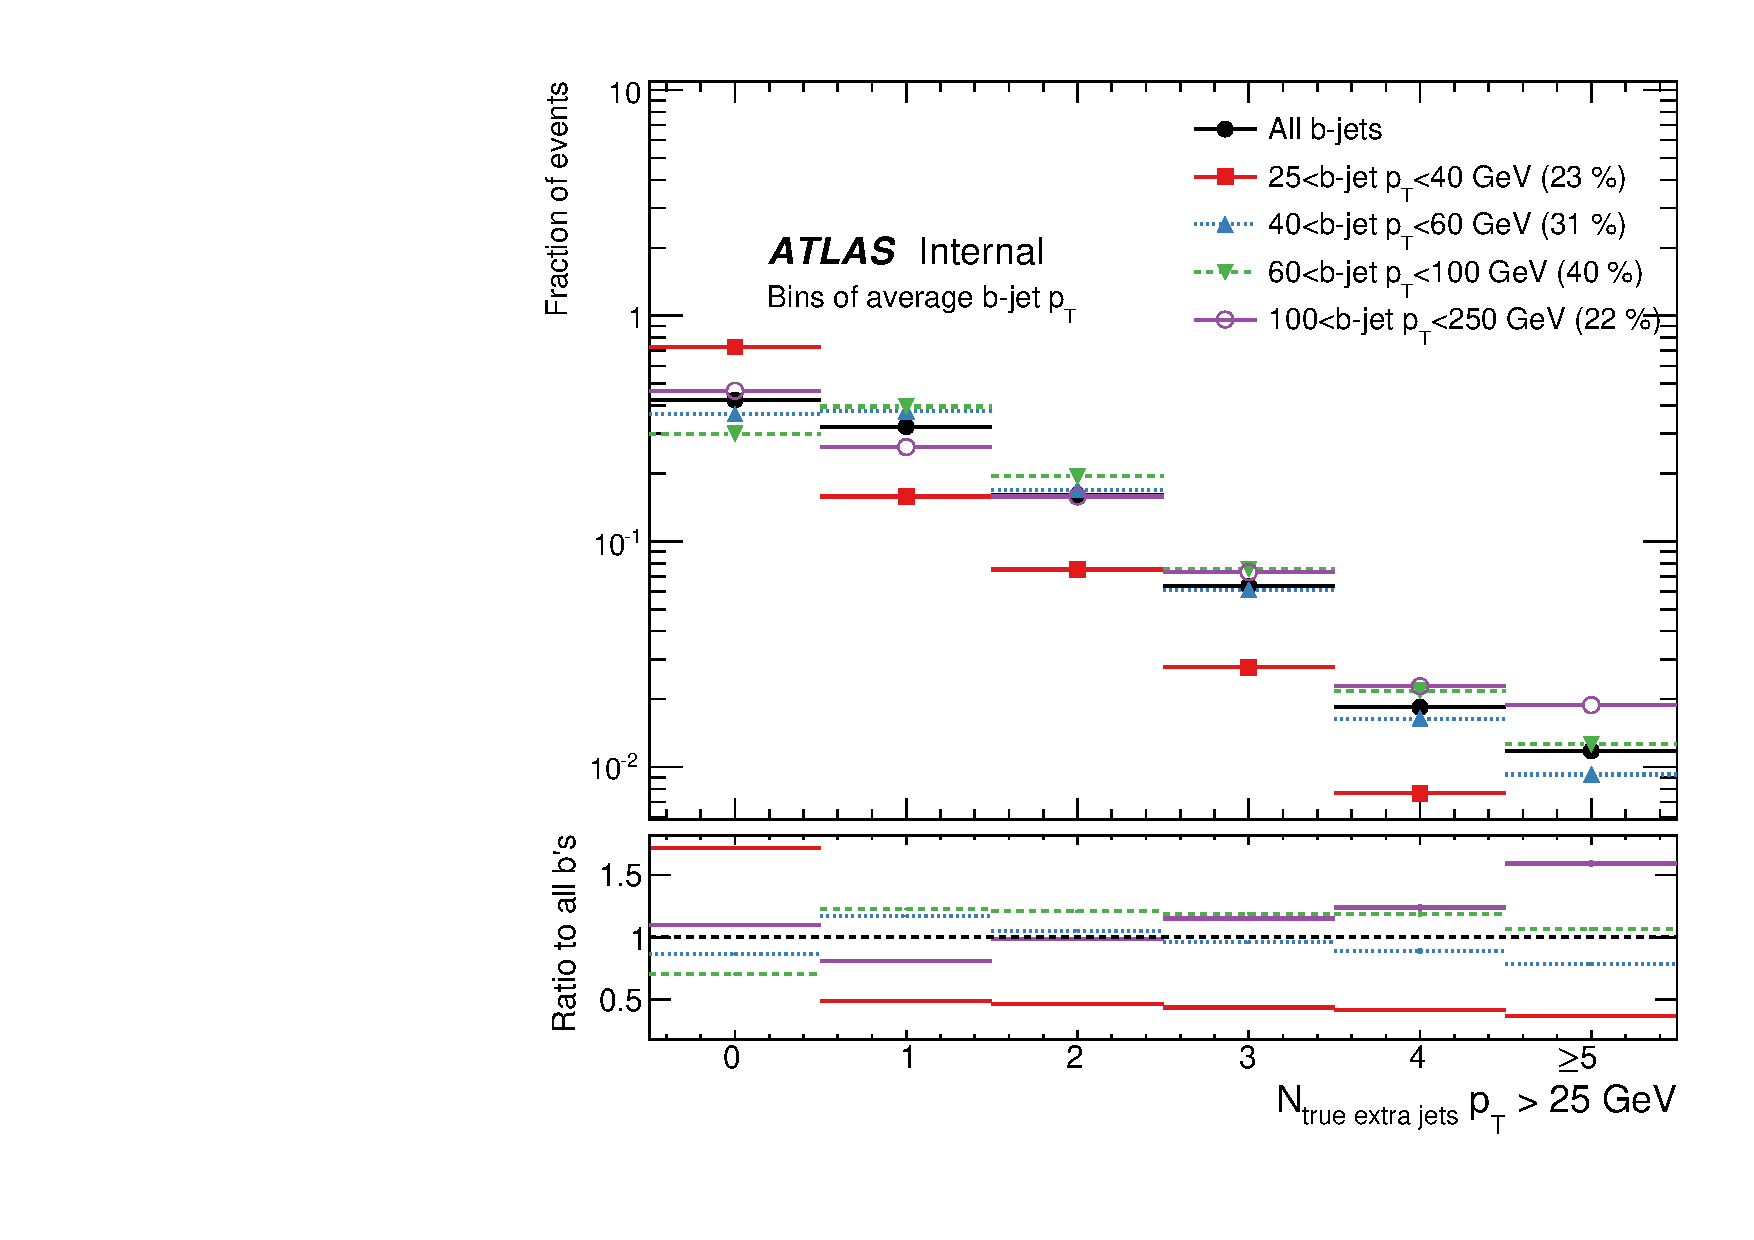
\includegraphics[width=\textwidth]{fig/TruthNotReco/BJetNJets25.pdf}
\end{subfigure}
~
\begin{subfigure}[]{0.45\textwidth}
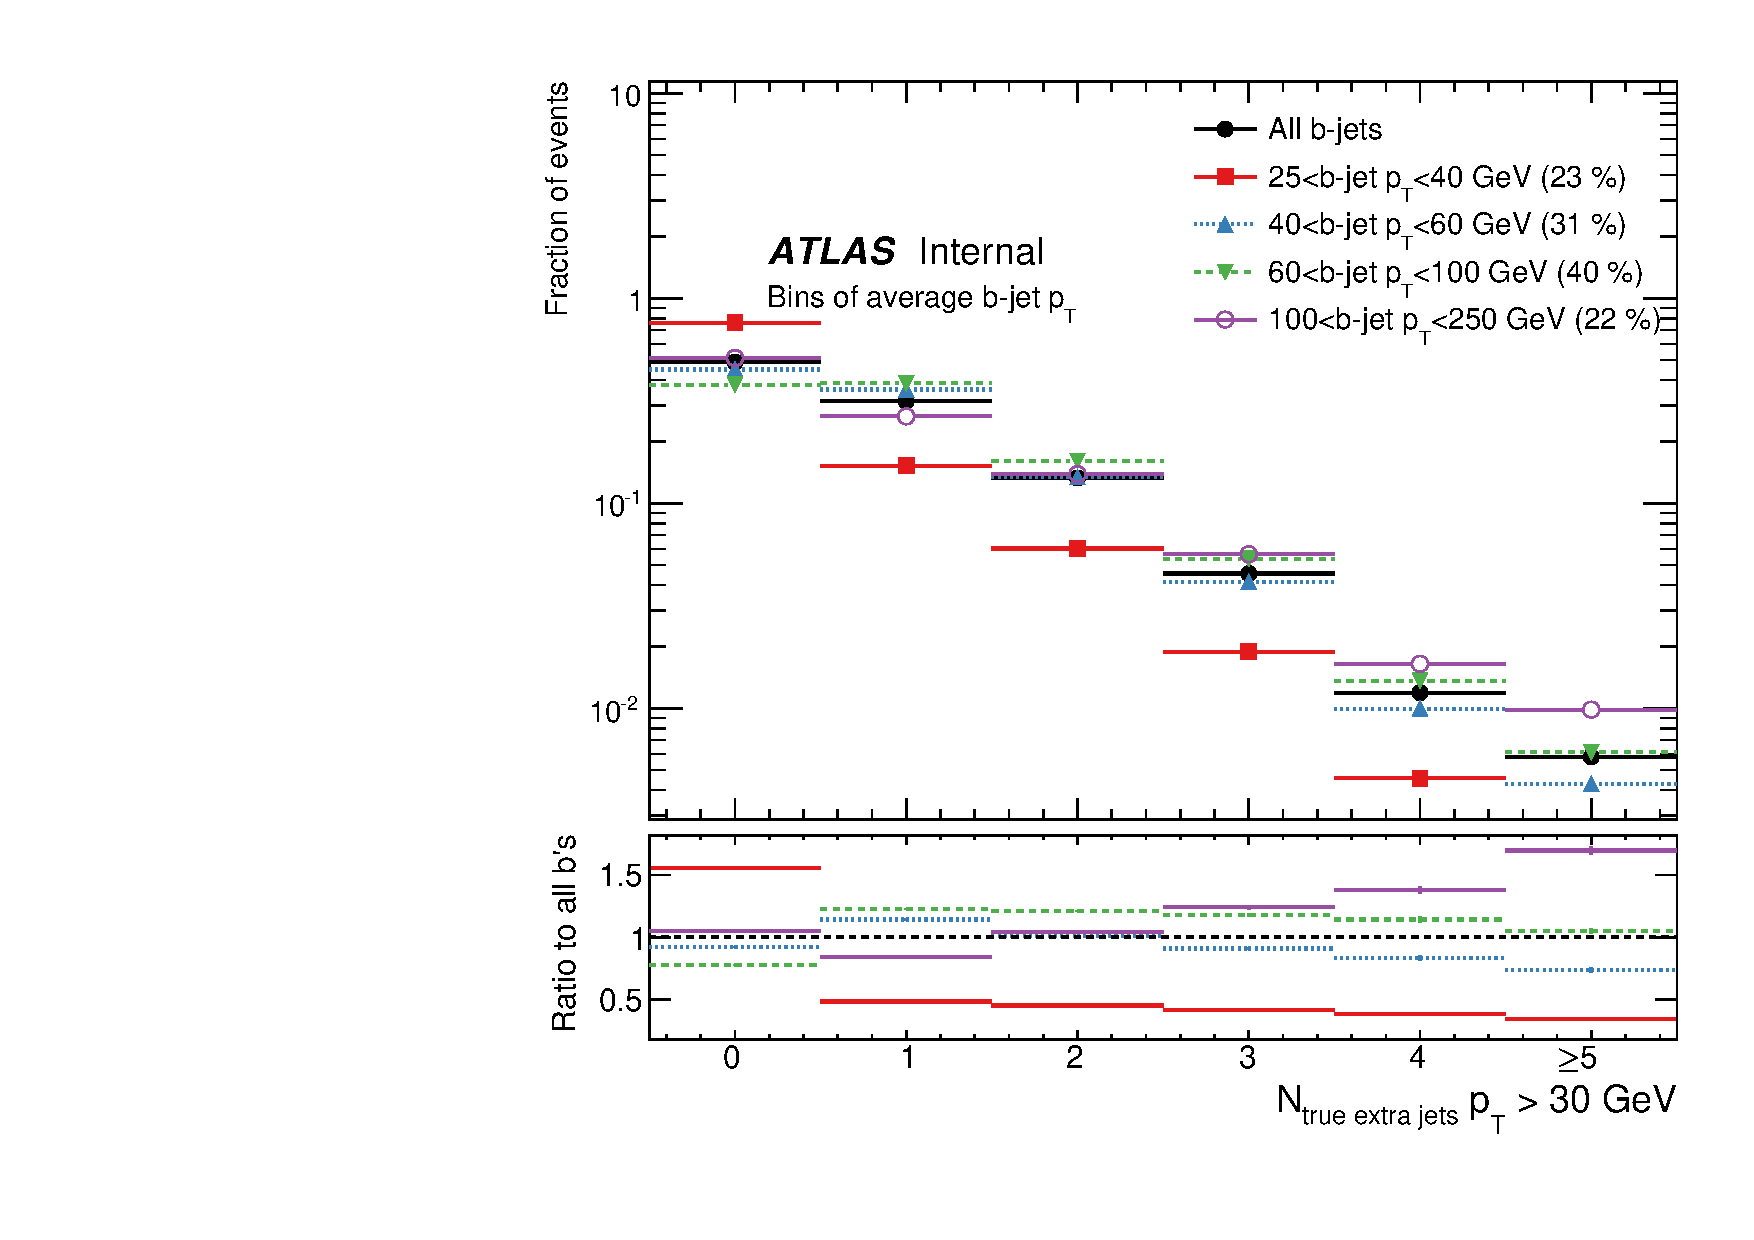
\includegraphics[width=\textwidth]{fig/TruthNotReco/BJetNJets30.pdf}
\end{subfigure}
~
\begin{subfigure}[]{0.45\textwidth}
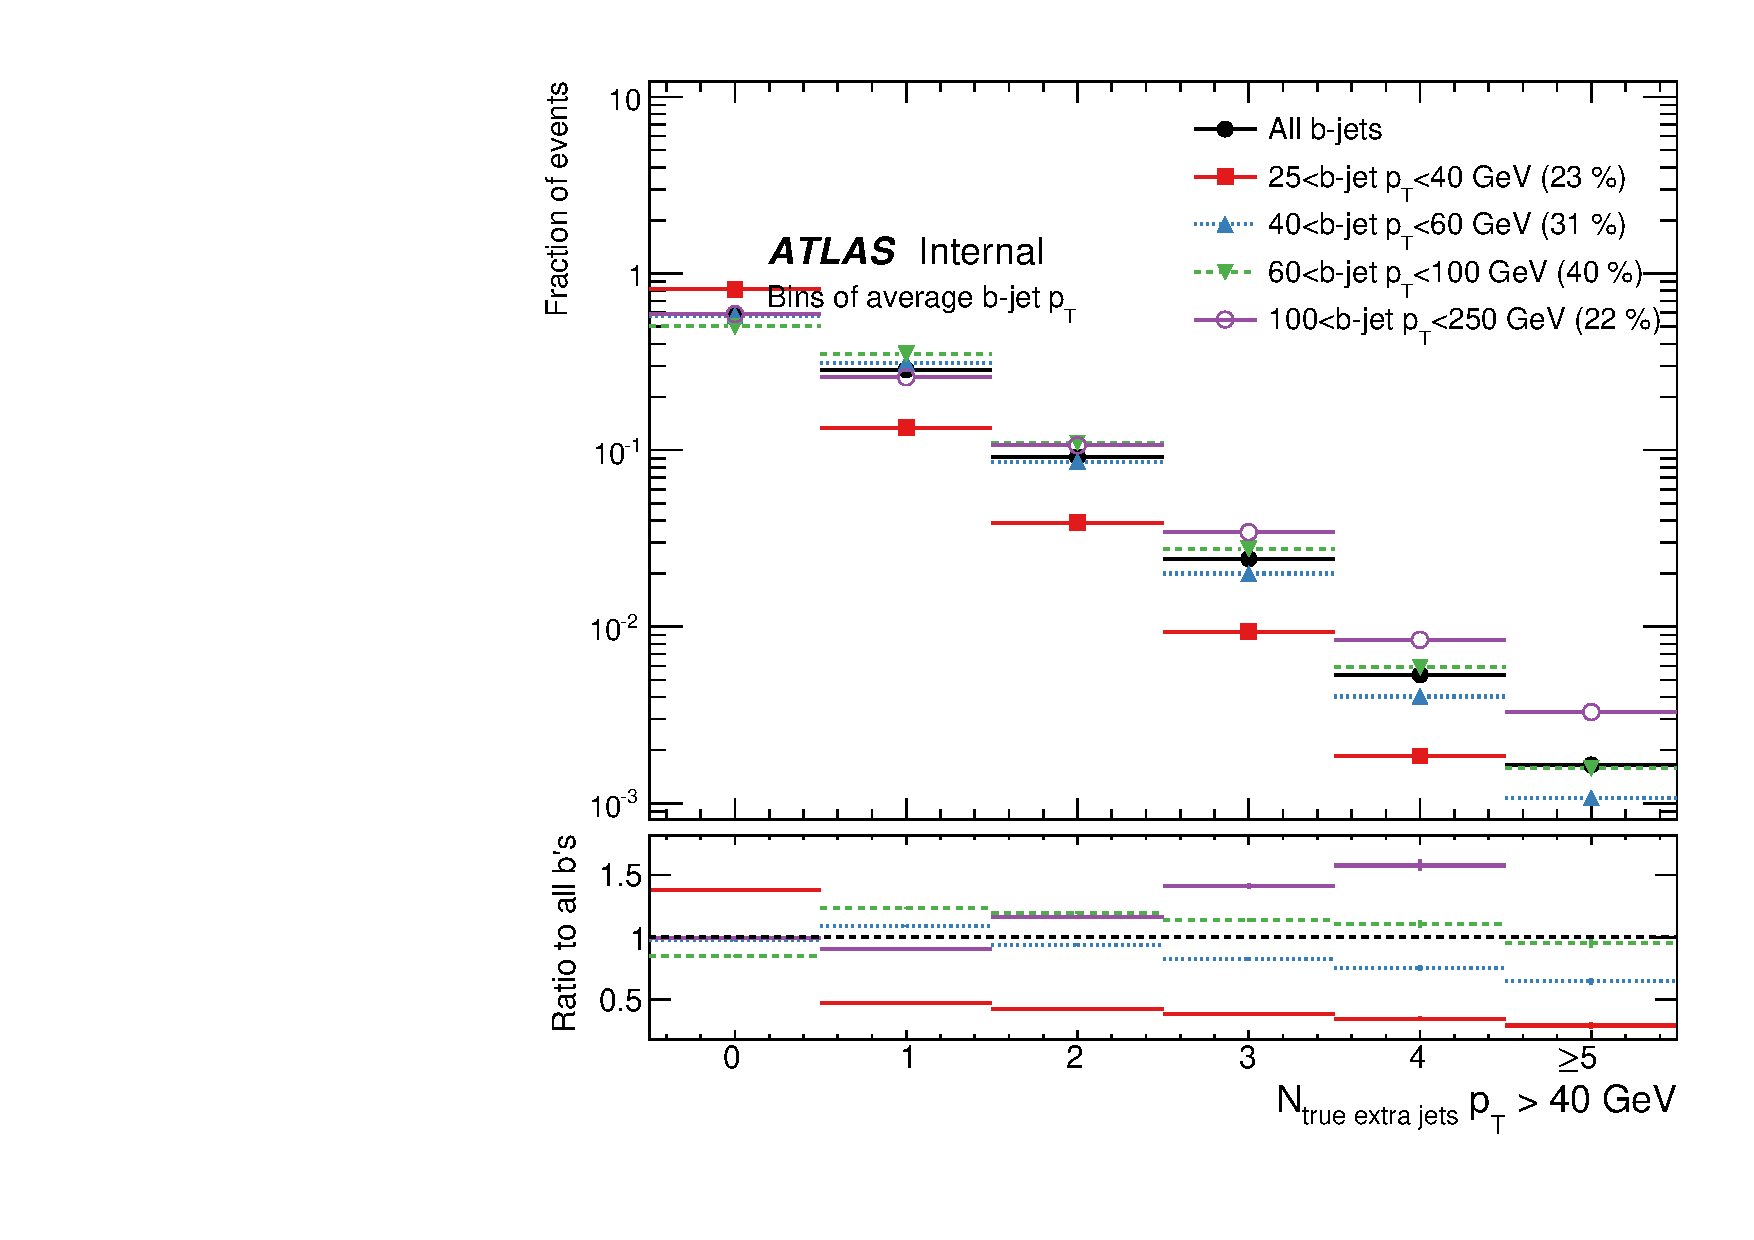
\includegraphics[width=\textwidth]{fig/TruthNotReco/BJetNJets40.pdf}
\end{subfigure}
~
\begin{subfigure}[]{0.45\textwidth}
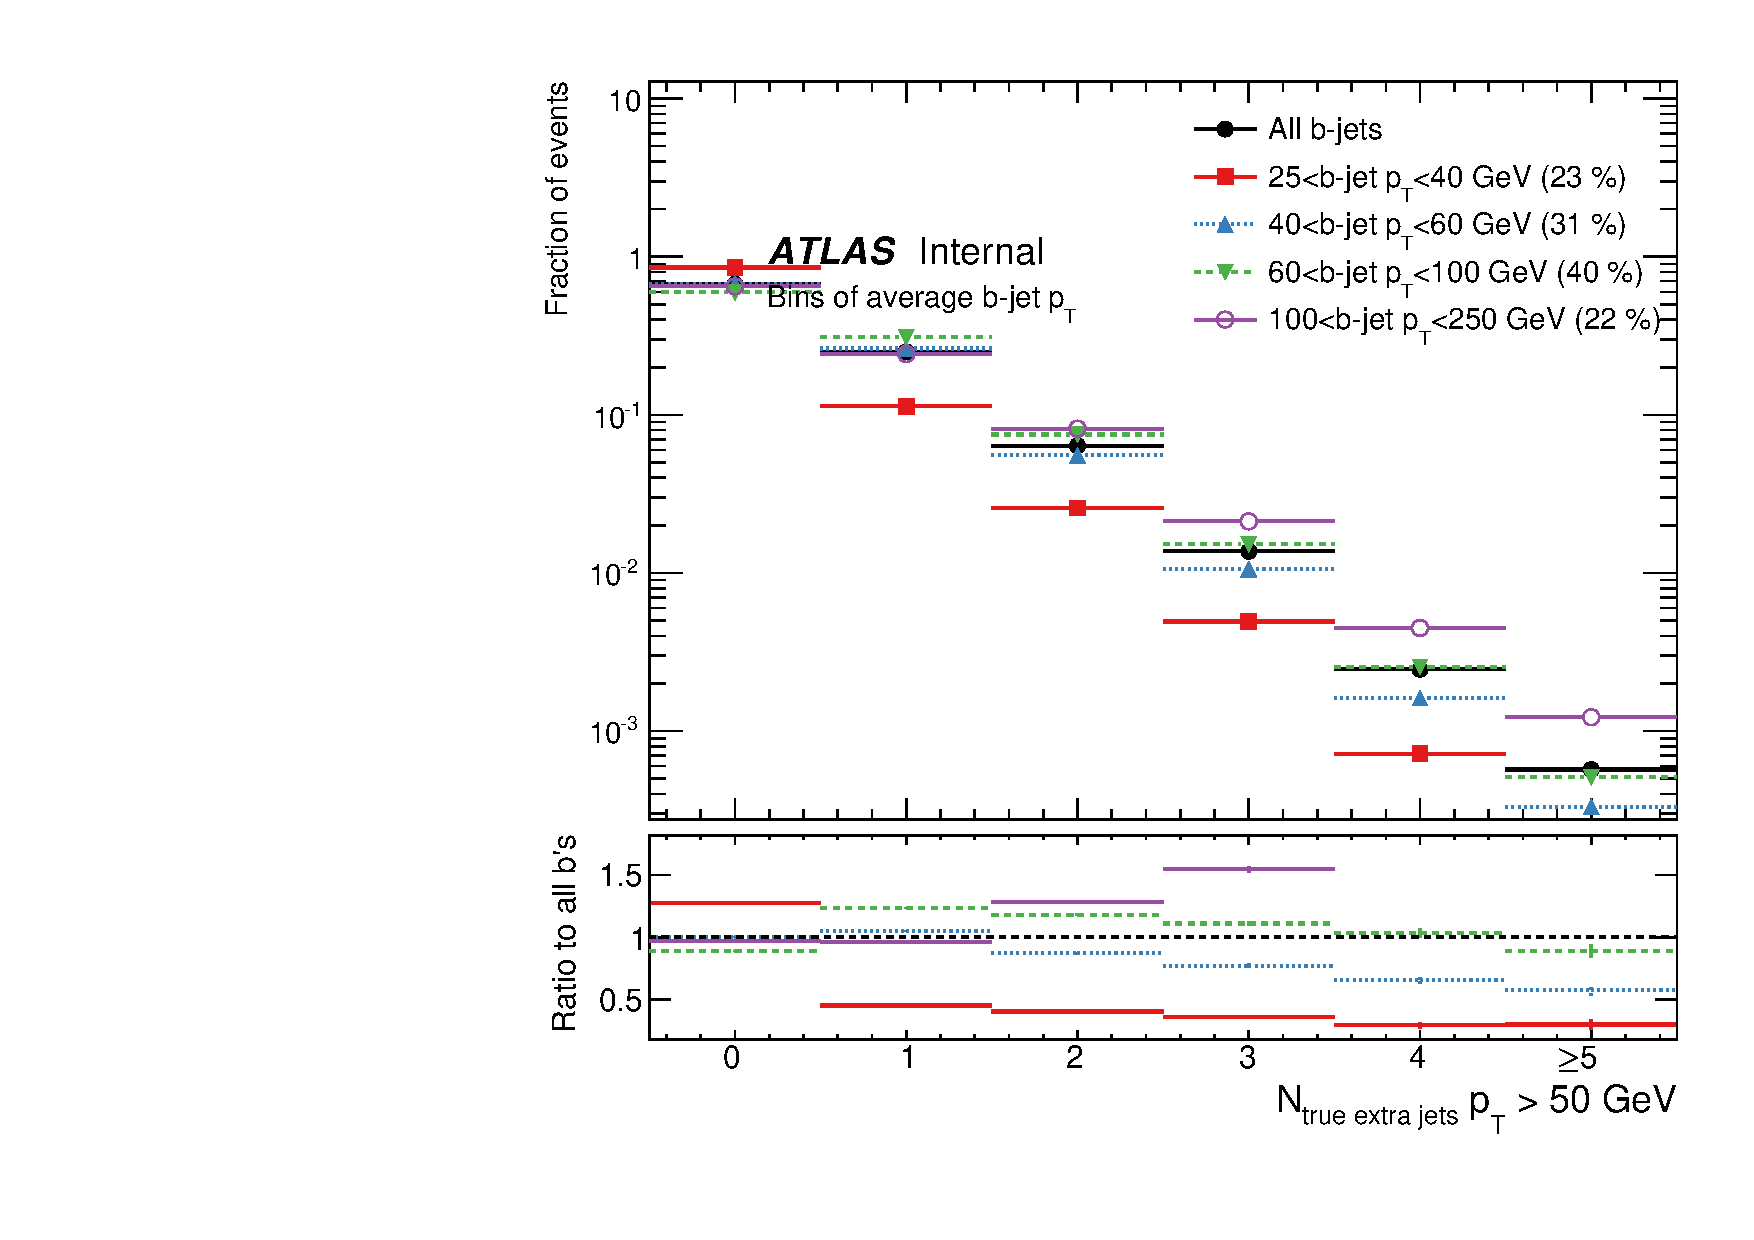
\includegraphics[width=\textwidth]{fig/TruthNotReco/BJetNJets50.pdf}
\end{subfigure}

\caption{Distributions of the number of extra truth jets with \pt > (a) 25, (b) 30, (c) 40 and (d) 50 \GeV, in bins of the average \pt of the 2 $b$-jets used to select the event. Each distribution is normalized by the number of events falling in that bin. The extra jet multiplicity decreases for softer $b$-jets due to lower $p_{T}^{\textrm{top}}$.}
\label{fig:truebextramult}

\end{figure}


\begin{figure}
\centering
\begin{subfigure}[]{0.33\textwidth}
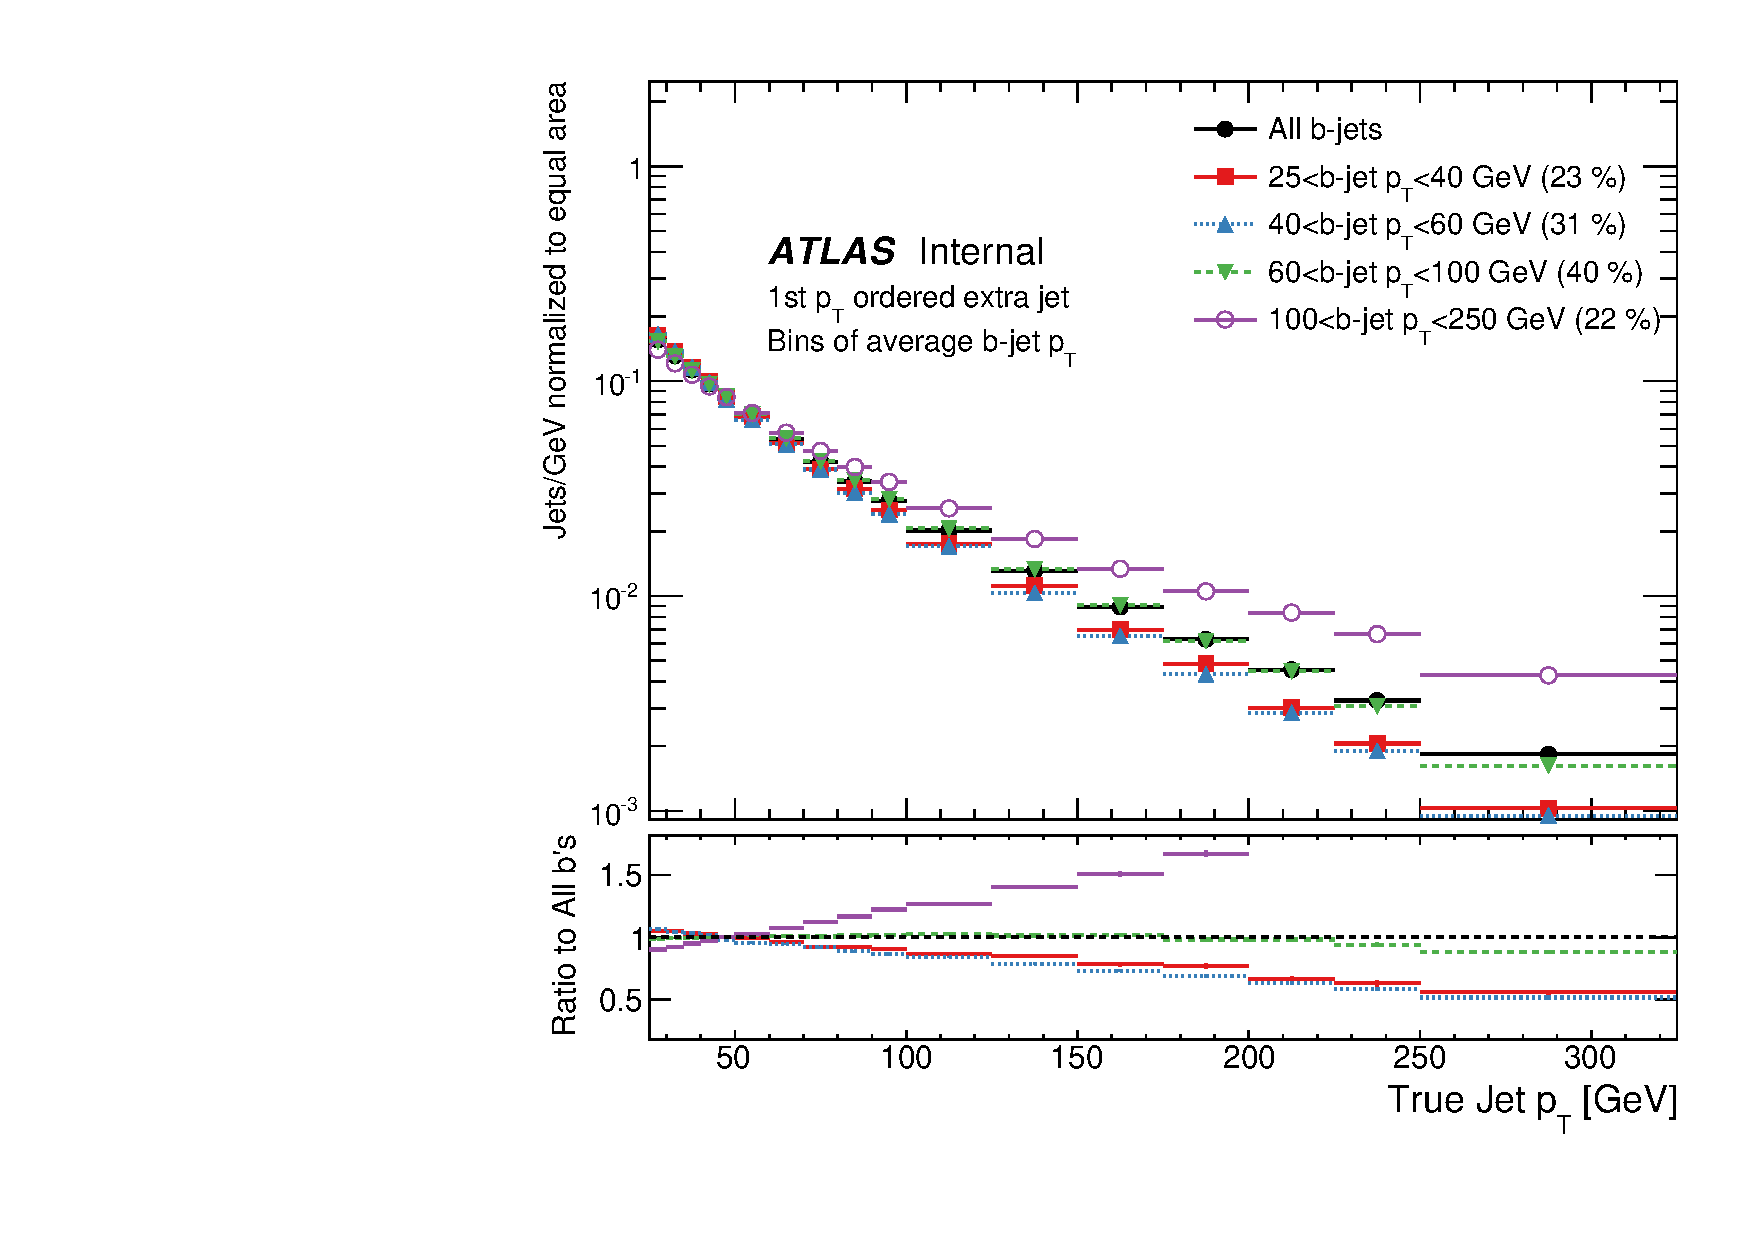
\includegraphics[width=\textwidth]{fig/TruthNotReco/BJetPtJet0.pdf}
\end{subfigure}
~
\begin{subfigure}[]{0.33\textwidth}
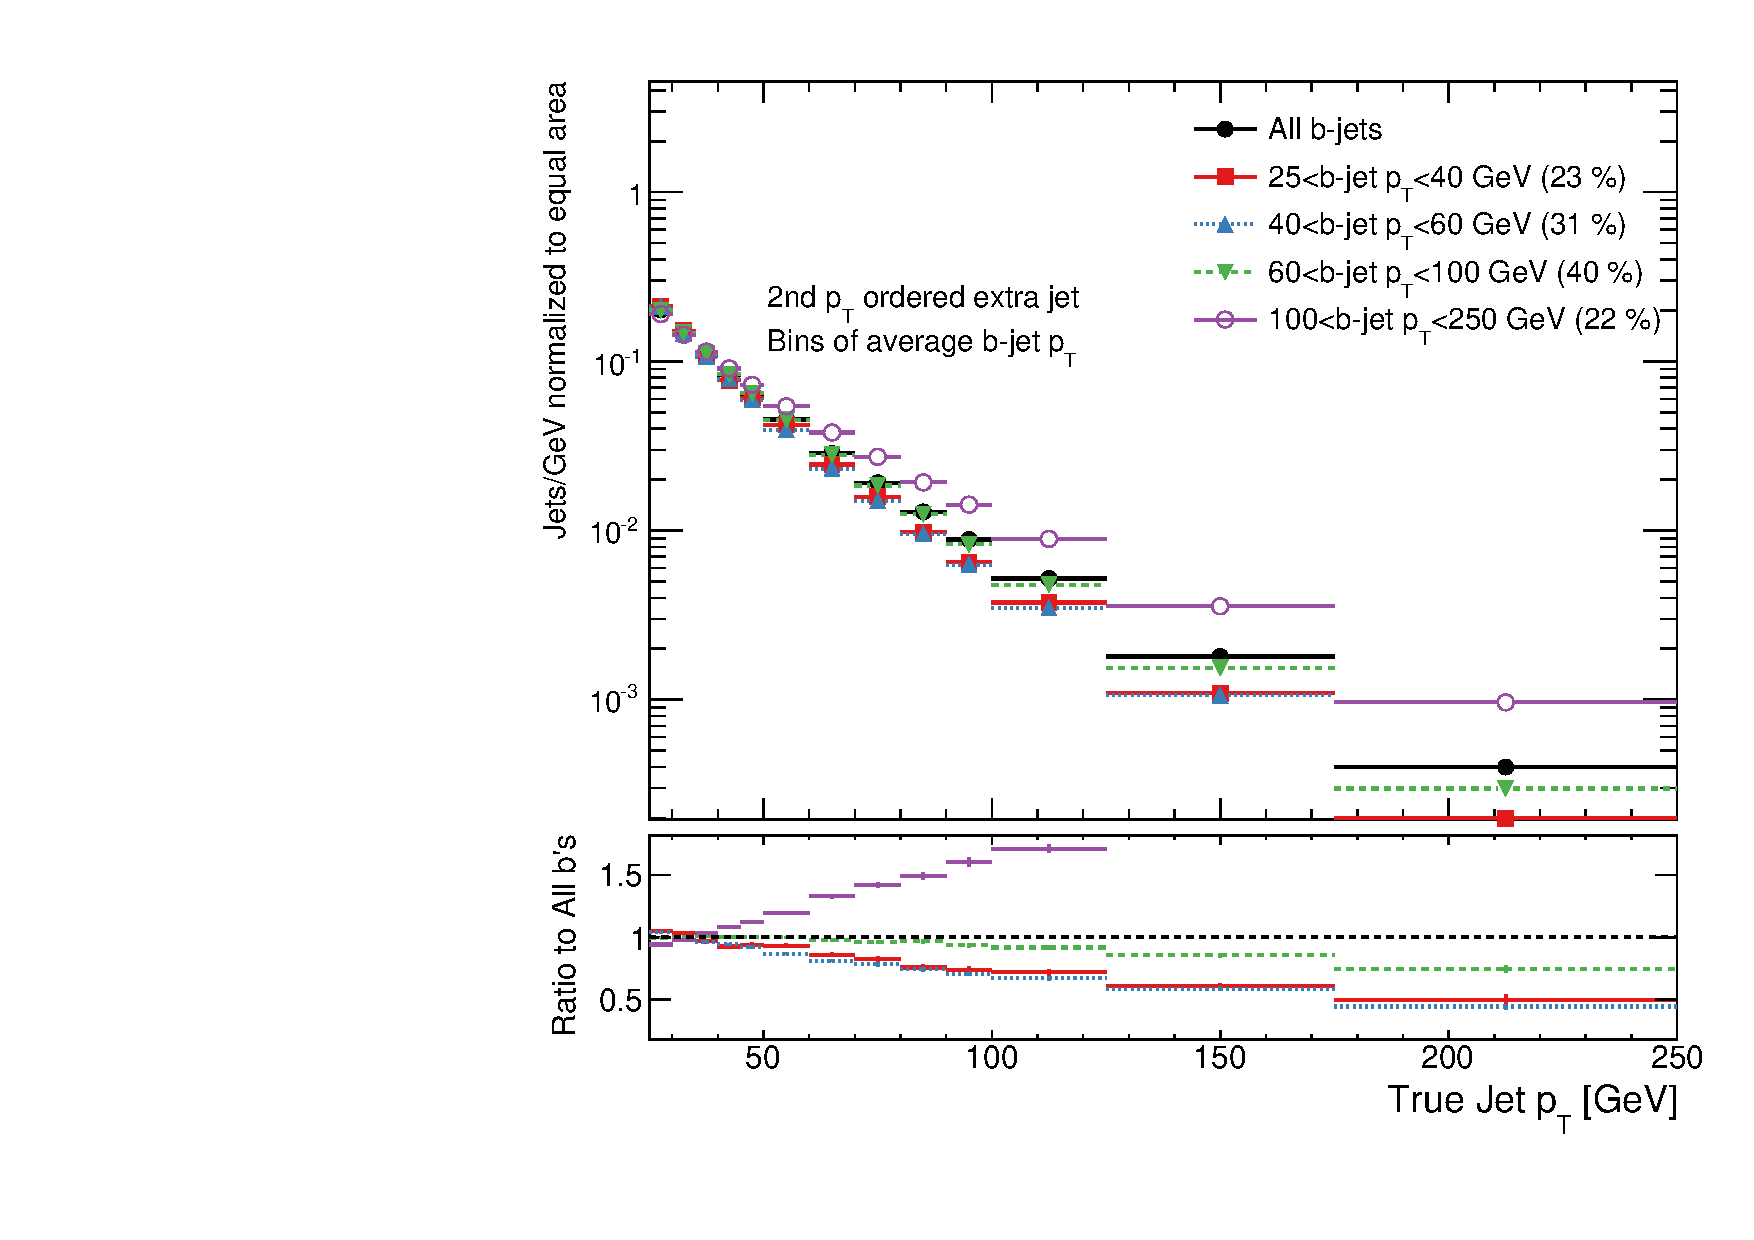
\includegraphics[width=\textwidth]{fig/TruthNotReco/BJetPtJet1.pdf}
\end{subfigure}
~
\begin{subfigure}[]{0.33\textwidth}
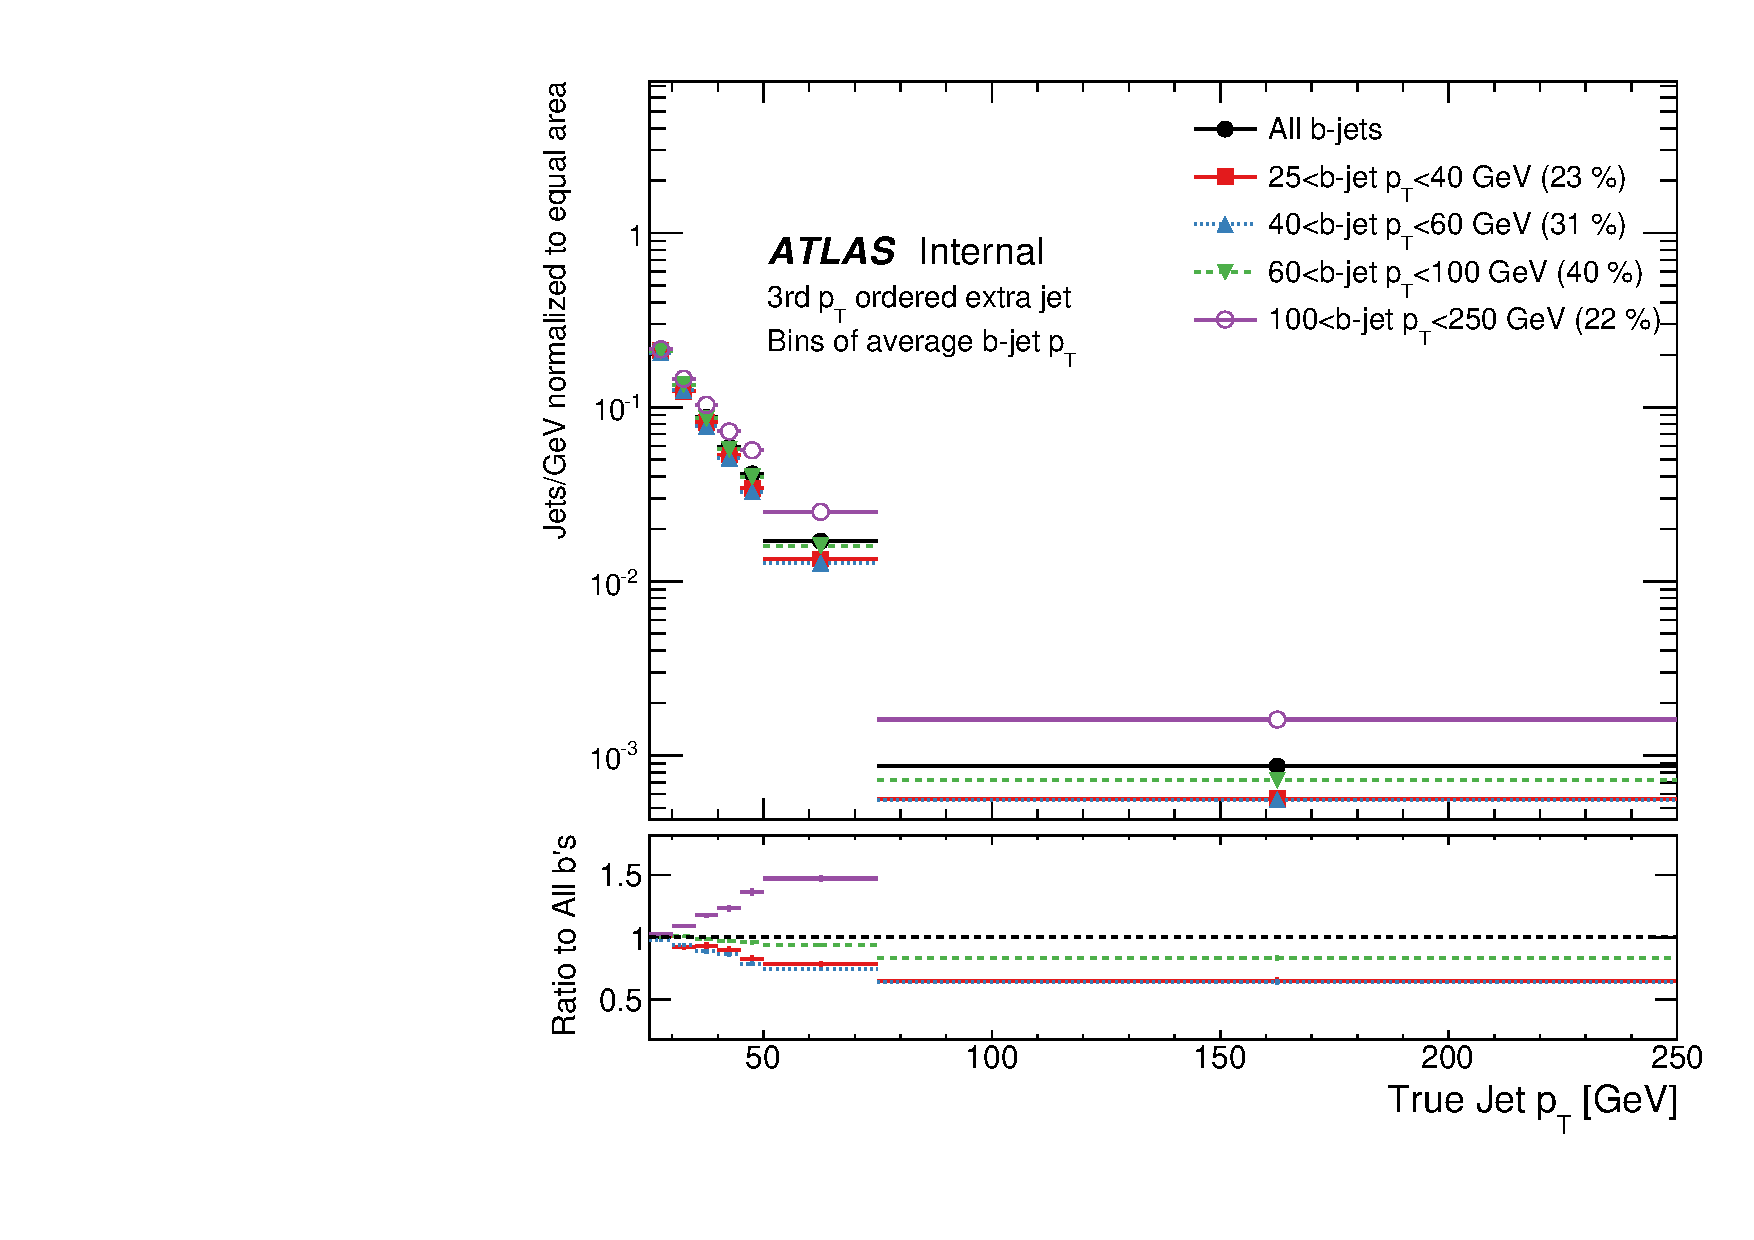
\includegraphics[width=\textwidth]{fig/TruthNotReco/BJetPtJet2.pdf}
\end{subfigure}
~
\begin{subfigure}[]{0.33\textwidth}
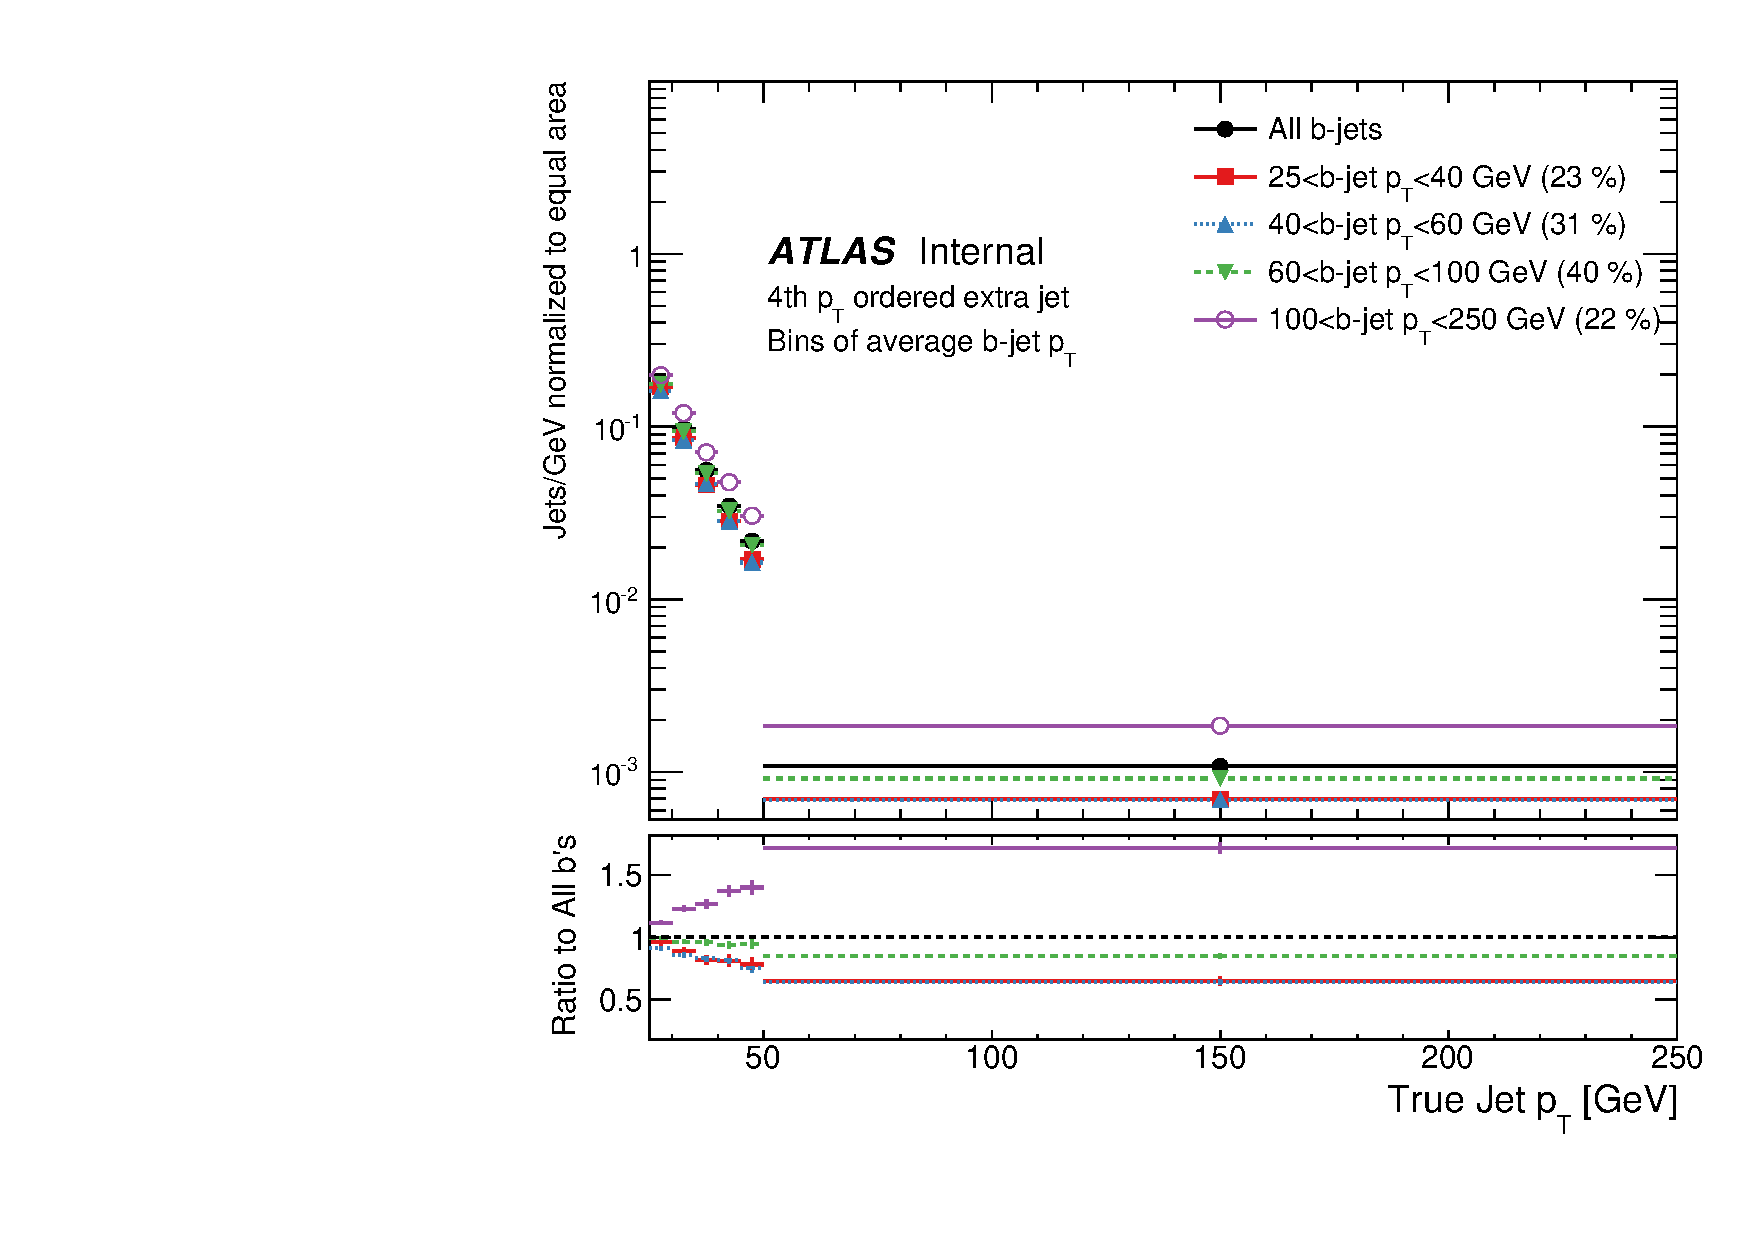
\includegraphics[width=\textwidth]{fig/TruthNotReco/BJetPtJet3.pdf}
\end{subfigure}
~
\begin{subfigure}[]{0.33\textwidth}
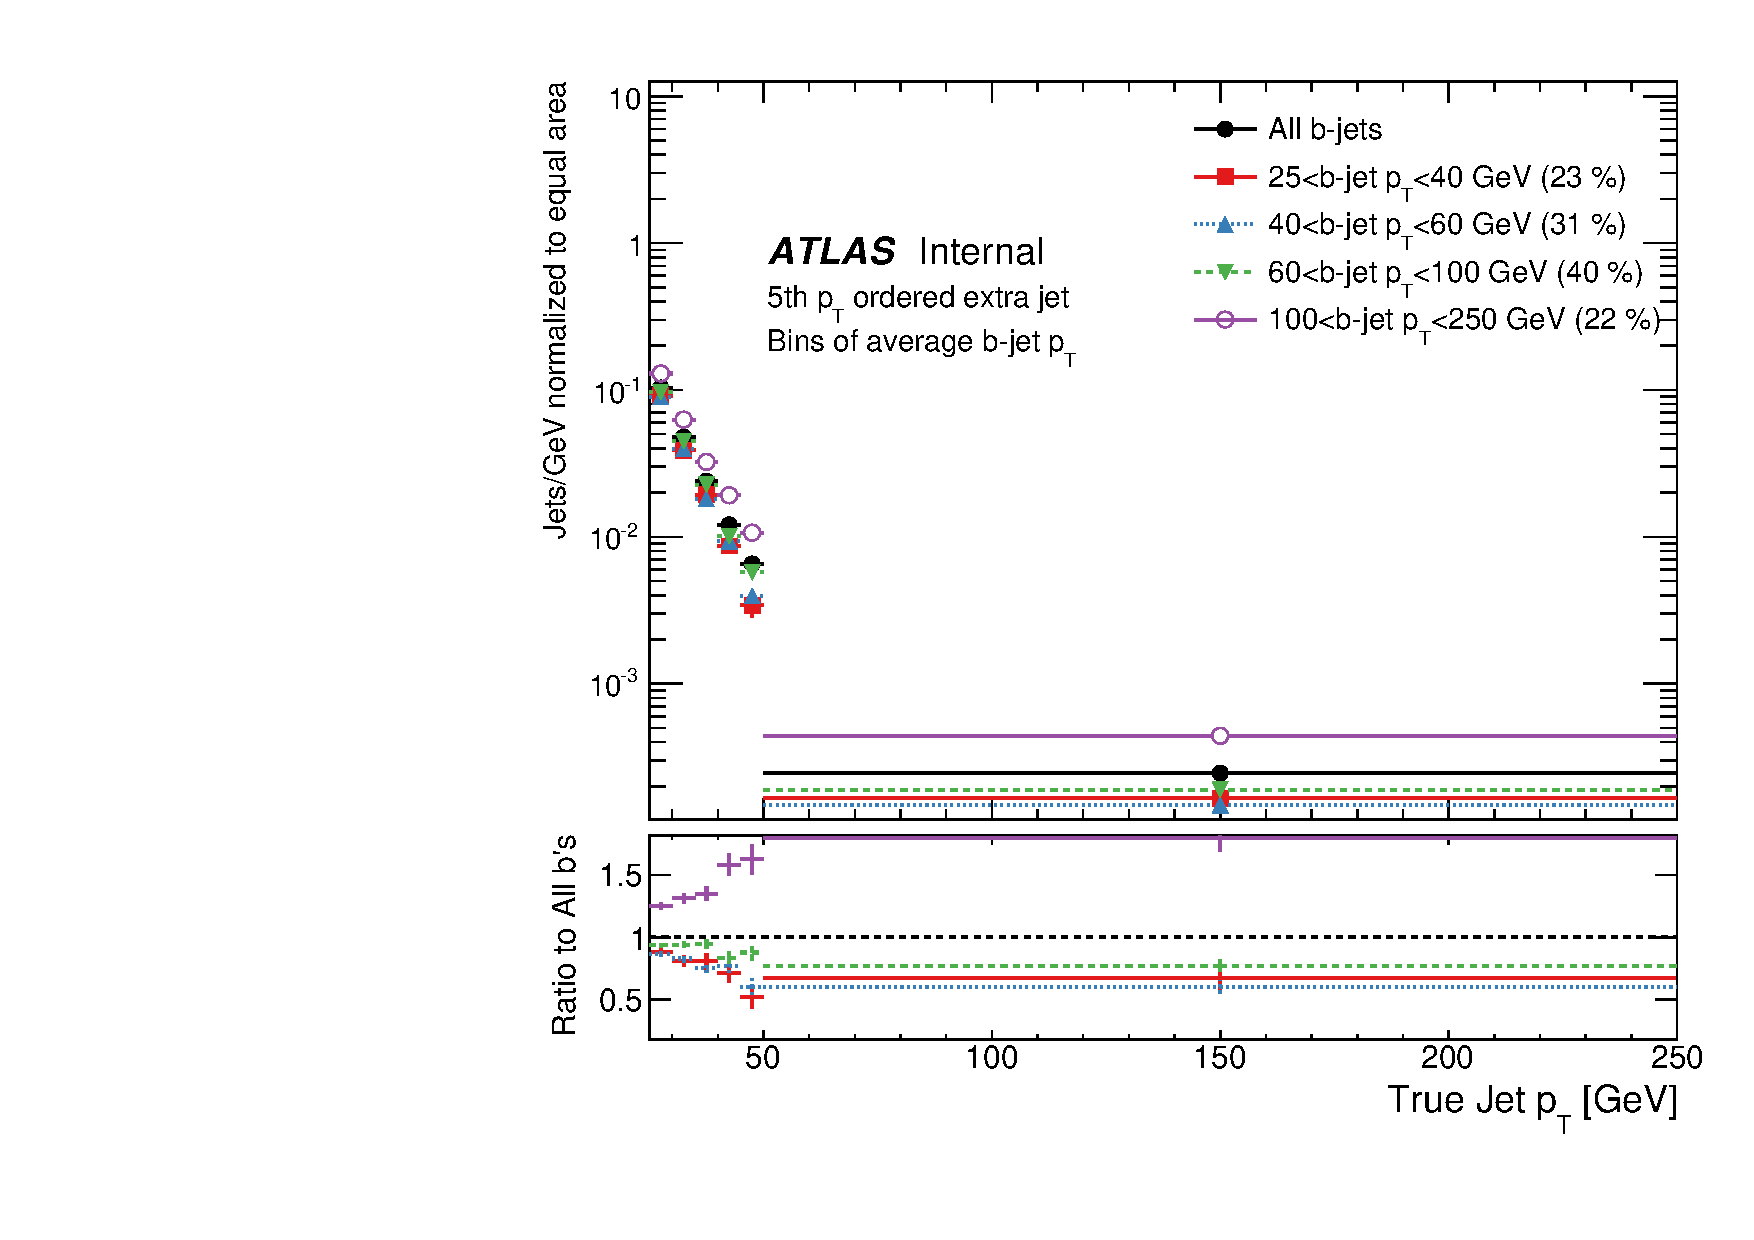
\includegraphics[width=\textwidth]{fig/TruthNotReco/BJetPtJet4.pdf}
\end{subfigure}

\caption{Distributions of the extra jet \pt for bins for jet ranks 1-5 (a-e), shown in bins the average \pt of the 2 $b$-jets used to select the event. Each distribution is normalized by the number of events falling in that bin. The extra jet \pt decreases for softer $b$-jets due to lower $p_{T}^{\textrm{top}}$.}
\label{fig:truebextrapt}
\end{figure}

\clearpage
